\chapter[Cloud Capacitor]{Cloud Capacitor}
\label{chap:capacitor}
% ----------------------------------------------------------
A partir da especificação do processo de avaliação de capacidade descrita no
capítulo anterior, bem como dos componentes de suporte a esse processo, apresentamos
a sua implementação na forma de um sistema computacional que demonstra seu funcionamento,
eficácia e eficiência.

Cloud Capacitor é um arcabouço para criação de sistemas de avaliação de 
capacidade em ambientes de nuvem de infraestrutura como serviço. Ele permite que 
sejam implementadas lógicas customizadas de avaliação do desempenho resultante
da execução da Aplicação sob Teste. Essas lógicas são então reconhecidas pelo Cloud 
Capacitor como Estratégias de Avaliação.

\begin{figure}[htb]
  \caption{\label{fig_arq_alto_nivel}Arquitetura de alto nível do Cloud Capacitor}
  \begin{center}
    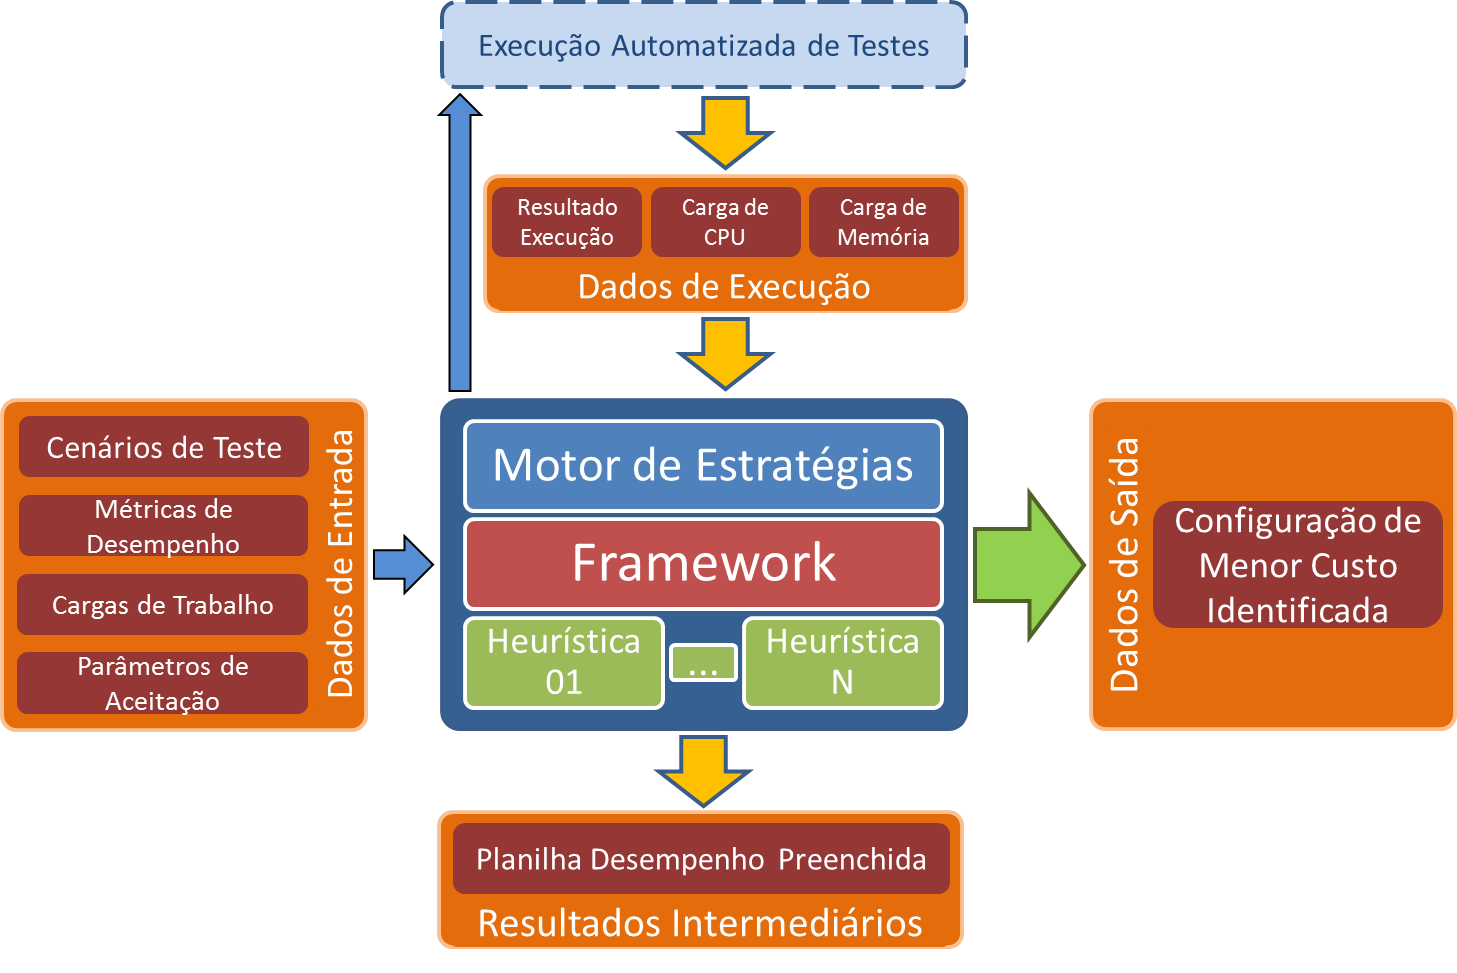
\includegraphics[scale=0.5]{img/arquiteturaAltoNivel}
  \end{center}
\end{figure}

****RASCUNHO
\subsection{Heuristicas}
Para que uma Heurística de Avaliação de Capacidade seja compatível no âmbito deste trabalho, 
deve apresentar um conjunto mínimo de operações esperadas para que a lógica da
avaliação se complete e o resultado final obtido possa ser considerado válido e
comparável com os resultados obtidos por outras Heurísticas.

Além disso, as operações constituem a interface pela qual o controlador das 
sessões de avaliação pode configurar as Heurísticas e informar-lhe os dados 
necessários ao controle da sua execução.
 
Apresentamos esse conjunto mínimo de operações nas subseções a seguir, que 
representam o arcabouço necessário para a construção de uma Heurística de 
Avaliação de Capacidade.
 
% ----------------------------------------------------------
